%%%%  Las secciones de texto con fórmulas se separan con %%%%
%% Las fórmulas presentes entre 2 secciones de texto se separan con %%

%%%%%%%%%%%%%%%
%%  Capítulo 1: Introducción  %%
%%%%%%%%%%%%%%%

%%%%
\section{Reseña histórica}
\label{sec_intro_resenia}
%%%%

\begin{table}[H]
\centering
\begin{tabular}{c|c|c|cc|c|}
\cline{2-6}
& \multicolumn{2}{c|}{Ancho de haz} & \multicolumn{2}{c|}{\multirow{2}{*}{$G_{fn}\left(\theta_0\right)\,$(dB)}} & \multirow{2}{*}{Relación frente}\\
& \multicolumn{2}{c|}{principal (grados)} & & & \multirow{2}{*}{espalda (dB)}\\
\cline{2-5}
& Plano E & Plano H & \multicolumn{1}{|c|}{Plano E} & Plano H &\\
\hline
\multicolumn{1}{|c|}{Simulación} & 82,90 & 81,02 & \multicolumn{1}{|c|}{-7,35} & -8,75 & 18,44\\
\hline
\multicolumn{1}{|c|}{Medición} & 82,37 & 85,22 & \multicolumn{1}{|c|}{-7,33} & -8,91 & 17,71\\
\hline
\end{tabular}
\caption{Comparación entre la simulación y la medición del ancho de haz principal, la ganancia normalizada en el ángulo $\theta_0$ y la relación frente-espalda.}
\label{tabla_mediciones:3}
\end{table}

%%%%
\begin{itemize}
\item En el año 1864 \cite{Baars}, una gran cantidad de evidencia experimental que fue acumulada por más de 150 años permitió al físico inglés James Clerk Maxwell establecer que los fenómenos electromagnéticos están gobernados por una serie de ecuaciones, conocidas posteriormente como ecuaciones de Maxwell.
\item La primera antena parabólica fue construida por el físico alemán Heinrich Hertz en el año 1888, y fue usada para demostrar experimentalmente la teoría electromagnética de Maxwell. La antena consistía en un reflector cilíndrico construido con una hoja metálica de zinc de 2 metros de longitud, 1,2 metros de ancho de abertura, una profundidad de 0,7 metros y excitado mediante un dipolo ubicado a lo largo de la línea focal que operaba a una frecuencia de 450 MHz. Los experimentos de Hertz significaron el comienzo del enorme desarrollo que tuvo la radio en el siglo 20, y también hizo que varios físicos e ingenieros de la época consideraran la posibilidad de que las ondas de radio puedan ser emitidas por el sol.
\item En el año 1930, el italiano Guglielmo Marconi utilizó un reflector parabólico para medir el alcance de una transmisión a 500 MHz en su barco sobre el Mar Mediterráneo, encontrando que se podían recibir señales a una distancia igual a cinco veces el alcance visual, descubriendo lo que se conocería posteriormente como enlaces troposféricos.
\item En el año 1932, el ingeniero estadounidense Karl Guthe Jansky, mientras estudiaba la interferencia en el sistema de radiotelefonía de onda corta, descubrió la radiación proveniente del núcleo galáctico. Inspirado en el descubrimiento de Jansky, el ingeniero estadounidense Grote Reber, a quien se lo considera pionero de la radioastronomía, construyó en el año 1937 la primera gran antena parabólica, con un diámetro de 9 metros, en el patio trasero de su casa. En el año 1940, Reber publicó el primer mapa de radio de la Vía Láctea.
\item La primera detección de un avión fue accidental. En el año 1930, el ingeniero estadounidense Lawrence A. Hyland del Naval Research Laboratory comprobó, mientras probaba un sistema DF (direction finding), que al pasar un avión por las cercanías se producía un incremento de la señal recibida. En Gran Bretaña se iniciaron los estudios sobre el radar  en el año 1934, cuando se propuso a Sir Robert Watson-Watt la construcción de un haz destructor con ondas de radio; las conclusiones del estudio fueron que no era viable, pero recomendaba estudiar el problema de la detección de aviones, lo que desencadenó en la creación del radar. El desarrollo del radar durante la Segunda Guerra Mundial proporcionó un gran impulso al estudio de las antenas parabólicas, y representó una gran ventaja táctica para la Royal Air Force en la Batalla de Inglaterra, que culminó con la derrota de la Luftwaffe.
\item Durante la década del 60, las antenas parabólicas comenzaron a ser ampliamente utilizadas en las redes de comunicaciones de microondas terrestres, las cuales transmitían llamadas telefónicas y programas de televisión a través de los continentes.
\item El 4 de Octubre del año 1947, la Unión Soviética lanzó el satélite Sputnik I; Estados Unidos reaccionó al reto soviético y se inició una carrera espacial. En el año 1962 se lanzó el satélite Telstar, el primero con repetidoras de banda ancha, y se construyó la primera antena parabólica utilizada para transmisiones satelitales en la estación terrena Goonhilly en Cornwall, Inglaterra, para comunicarse con el satélite Telstar. En el mismo año y mediante el mismo satélite, fue transmitida la primera señal de TV desde Estados Unidos hacia Europa.
\item La primera antena Cassegrain fue desarrollada en Japón en el año 1963 por NTT, KDDI y Mitsubishi Electric, y fue usada en octubre del mismo año en los primeros experimentos de retransmisión de TV por satélite a través del océano Pacífico. Esta antena, que basa su diseño en un telescopio reflector desarrollado en el año 1672 por el sacerdote francés Laurent Cassegrain, está conformada por un reflector principal cóncavo con forma de paraboloide y un reflector secundario convexo con forma de hiperboloide; las ondas radiadas por el alimentador, el cual está montado en la superficie del reflector principal, se reflejan primero en el reflector secundario y luego en el reflector principal. Se utiliza fundamentalmente en estaciones terrenas y en aplicaciones de radioastronomía.
\item La aparición en la década del 70 de herramientas de diseño por computadora, como NEC, capaces de determinar los diagramas de radiación de las antenas parabólicas, ha llevado al desarrollo de sofisticados diseños asimétricos, de múltiples reflectores y de múltiples alimentadores.
\end{itemize}
%%%%

%%%%
\section{Parámetros básicos de las antenas}
\label{sec_intro_param_basicos}
%%%%

%%%%
\subsection{Potencia media radiada y densidad de potencia media}
\label{subsec_intro_pot_med_rad}
%%%%

El vector de Poynting instantáneo describe la potencia asociada con una onda electromagnética, y se define como:
%%%%
\begin{align}
\mathbf{N} = \mathbf{E}\prodvec\mathbf{H}
\label{ec_intro:1}
\end{align}
%%%%
donde:
%%%%
\begin{align*}
\mathbf{N} &= \text{Vector de Poynting instantáneo (W/m$^2$).}\\
\mathbf{E} &= \text{Campo eléctrico instantáneo (V/m).}\\
\mathbf{H} &= \text{Campo magnético instantáneo (A/m).}
\end{align*}
%%%%
Como el vector de Poynting es una densidad de potencia, es posible obtener la potencia que atraviesa una superficie cerrada integrando la componente normal del vector de Poynting sobre la totalidad de la superficie.
%%%%
\begin{align}
P = \oiint\limits_{S}\mathbf{N}\prodesc d\mathbf{s} = \oiint\limits_{S}\mathbf{N}\prodesc\versor{n}\,ds
\label{ec_intro:2}
\end{align}
%%%%
donde:
%%%%
\begin{align*}
P &= \text{Potencia total instantánea (W).}\\
\versor{n} &= \text{Versor normal a la superficie.}\\
ds &= \text{Area infinitesimal de la superficie cerrada (m$^2$).}
\end{align*}
%%%%
Para muchas aplicaciones es deseable hallar la densidad de potencia media, que se obtiene integrando el vector de Poynting instantáneo sobre un período y dividiendo por un período. A tal efecto y considerando que los campos son armónicos, se define la \emph{densidad de potencia media} a partir del valor medio del vector de Poynting.
%%%%
\begin{align}
\mathbf{W}_{av} = \left<\mathbf{N}\right> = \frac{1}{2}\,\Re\left(\mathbf{E}\prodvec\mathbf{H}^*\right)
\label{ec_intro:3}
\end{align}
%%%%
El factor $\frac{1}{2}$ aparece en la expresión \eqref{ec_intro:3} debido a que $\mathbf{E}$ y $\mathbf{H}$ representan valores pico y es necesario expresar los campos en valores RMS. La densidad de potencia media asociada con los campos electromagnéticos de la antena en la región de campo lejano es predominantemente activa, motivo por el cual la definición del valor medio del vector de Poynting contempla solamente la parte real; la parte imaginaria representa la densidad de potencia reactiva asociada con los campos electromagnéticos, que es prácticamente nula en la región de campo lejano.

A partir de la definición \eqref{ec_intro:2}, la \emph{potencia media radiada} o simplemente \emph{potencia radiada} puede expresarse como:
%%%%
\begin{align}
P_{rad} = \!\iint\limits_{S}\mathbf{W}_{av}\prodesc\versor{n}\,ds
\label{ec_intro:4}
\end{align}
%%%%
Para observaciones de campo lejano la superficie cerrada puede ser cualquiera; por conveniencia matemática, se adopta una esfera centrada en el centro de la antena. La potencia radiada por la antena, entonces, queda expresada como:
%%%%
\begin{align}
P_{rad} = \!\int_0^{\,2\pi}\!\int_0^{\,\pi}\!W_{av}\,r^2\sen\theta\,d\theta\,d\phi
\label{ec_intro:5}
\end{align}
%%%%

%%%%
\subsection{Intensidad de radiación}
\label{subsec_intro_int_rad}
%%%%

Dado que la densidad de potencia media depende de la distancia, se acostumbra a definir la \emph{intensidad de radiación} como el producto de la densidad de potencia media por el cuadrado de la distancia, con el fin de obtener una magnitud independiente de la distancia.
%%%%
\begin{align}
U = W_{av}\,r^2
\label{ec_intro:6}
\end{align}
%%%%
Para campo lejano, la intensidad de radiación está relacionada con el campo eléctrico de la antena por:
%%%%
\begin{align}
U\left(\theta,\phi\right) &\simeq \frac{r^2}{2\eta}\left[\lvert E_{\theta}\left(\theta,\phi\right)\rvert^2 + \lvert E_{\phi}\left(\theta,\phi\right)\rvert^2\right]
\label{ec_intro:7}
\end{align}
%%%%
donde:
%%%%
\begin{align*}
E_{\theta}, E_{\phi} &= \text{Componentes del campo eléctrico de la antena para campo lejano (V/m).}\\
\eta &= \text{Impedancia intrínseca del medio ($\Omega$).}
\end{align*}
%%%%
La componente radial del campo eléctrico $E_r$ es muy pequeña para observaciones de campo lejano, por lo que se desprecia.

La potencia radiada se obtiene integrando la intensidad de radiación sobre el elemento de ángulo sólido, por lo que:
%%%%
\begin{align}
P_{rad} = \iint\limits_{\Omega}Ud\Omega = \!\int_0^{\,2\pi}\!\int_0^{\,\pi}\!U\sen\theta\,d\theta\,d\phi
\label{ec_intro:8}
\end{align}
%%%%
donde $d\Omega$ = Elemento de ángulo sólido = $\sen\theta\,d\theta\,d\phi$.
%%%%

%%%%
\subsection{Diagrama de radiación}
\label{subsec_intro_diag_rad}
%%%%

%%%%
Se define al \emph{diagrama de radiación} como una representación gráfica de las propiedades de radiación en función de las coordenadas espaciales. Generalmente, el diagrama de radiación de una antena es un diagrama tridimensional o un grupo de secciones sobre planos determinados por los ángulos $\uptheta$ y $\upphi$.

En la práctica, generalmente se emplean los diagramas de radiación de potencia en dB. Muchas veces se trabaja con diagramas de potencia normalizados, con el fin de poder comparar las características de radiación de distintos tipos de antenas. La representación de los diagramas de radiación puede realizarse tanto en coordenadas polares como en coordenadas cartesianas, como puede observarse en la figura \ref{grup_fig_intro:1}.
%%%%
\begin{figure} [H]
\centering 
\subfigure[Representación polar del diagrama de radiación.]{
\label{fig_intro:1}
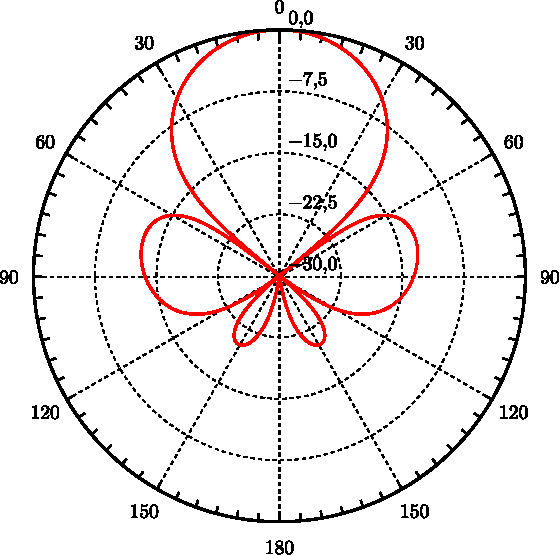
\includegraphics[scale = 1]{Figures/Intro/intro_1.pdf}}
\subfigure[Representación cartesiana del diagrama de radiación.]{
\label{fig_intro:2}
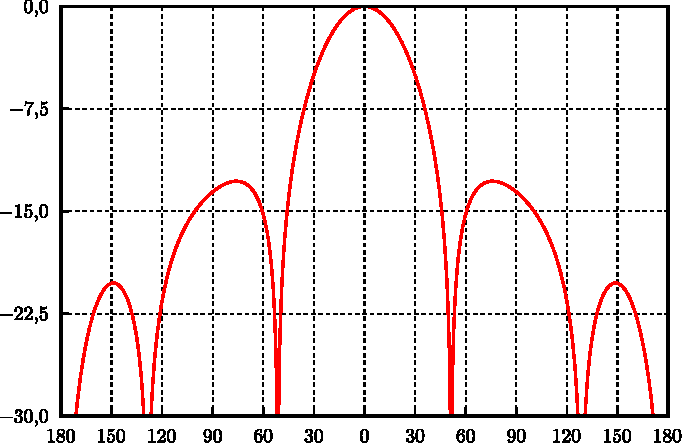
\includegraphics[scale = 1]{Figures/Intro/intro_2.pdf}}
\caption{Diagramas de radiación (dB).}
\label{grup_fig_intro:1}
\end{figure}
%%%%
Puede observarse en los diagramas de radiación una serie de lóbulos, donde es posible diferenciar los \emph{lóbulos principales}, en las direcciones de máxima radiación, y los \emph{lóbulos secundarios} o \emph{laterales}. Los lóbulos principales se definen por:
%%%%
\begin{itemize}
\item Amplitud.
\item Ancho de haz de potencia media (HPBW, \emph{Half-Power Beamwidth}): Ángulo en el que la densidad de potencia del lóbulo cae a la mitad de su valor máximo.
\item Ancho de haz entre ceros (FNBW, \emph{First-Null Beamwidth}): Separación angular entre los ceros del lóbulo.
\end{itemize}
%%%%
En el diagrama de radiación de la figura \ref{fig_intro:3} se señalan los anchos de haz de potencia media y entre ceros.
%%%%
\begin{figure} [H]
\centering 
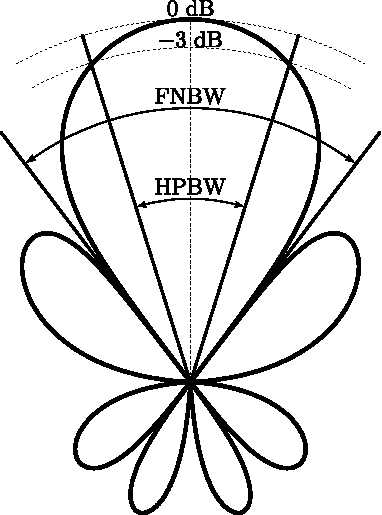
\includegraphics[scale = 1]{Figures/Intro/intro_3.pdf}
\caption{Anchos de haz de potencia media y entre ceros.}
\label{fig_intro:3}
\end{figure}
%%%%

%%%%
\subsection{Directividad}
\label{subsec_intro_direc}
%%%%

%%%%
La \emph{directividad} se define como la relación entre la intensidad de radiación en una determinada dirección que produce un elemento radiante en el espacio y la intensidad de radiación promedio, o sea, la intensidad de radiación producida por un foco isotrópico alimentado con la misma potencia.
%%%%
\begin{align}
D = \frac{U}{U_0}
\label{ec_intro:9}
\end{align}
%%%%
Un radiador isotrópico es una fuente ideal cuya potencia radiada es uniforme en todas las direcciones. Si bien no existe en la práctica, proporciona una referencia isotrópica con la cual se compararán otras antenas. Debido a su radiación simétrica, el vector de Poynting no será función de los ángulos $\uptheta$ y $\upphi$, y tendrá solamente una componente radial. Su potencia total radiada está dada por:
%%%%
\begin{align}
P_{rad} = \oiint\limits_{S}\mathbf{W}_0\prodesc d\mathbf{s} = \!\int_0^{\,2\pi}\!\int_0^{\,\pi}\!W_0r^2\sen\theta\,d\theta\,d\phi = 4\pi r^2W_0
\label{ec_intro:10}
\end{align}
%%%%
y la densidad de potencia por:
%%%%
\begin{align}
W_0 = \frac{P_{rad}}{4\pi r^2}
\label{ec_intro:11}
\end{align}
%%%%
A partir de la expresión \eqref{ec_intro:11}, se determina la intensidad de radiación del radiador isotrópico.
%%%%
\begin{align}
U_0 = W_0r^2 = \frac{P_{rad}}{4\pi}
\label{ec_intro:12}
\end{align}
%%%%
La directividad, entonces, queda definida como:
%%%%
\begin{align}
D = 4\pi\frac{U}{P_{rad}}
\label{ec_intro:13}
\end{align}
%%%%
Si no se especifica la dirección, queda implícito que la dirección es la de máxima intensidad de radiación, quedando la directividad máxima expresada como:
%%%%
\begin{align}
D_0 = D_{max} = 4\pi\frac{U_{max}}{P_{rad}}
\label{ec_intro:14}
\end{align}
%%%%
Si la antena no es isotrópica, no radiará uniformemente en todas las direcciones y, por lo tanto, la intensidad de radiación dependerá de los ángulos $\uptheta$ y $\upphi$; entonces, puede expresarse la intensidad de radiación como:
%%%%
\begin{align}
&U = B_0F\left(\theta,\phi\right) \simeq \frac{r^2}{2\eta}\left[\lvert E_{\theta}\left(\theta,\phi\right)\rvert^2 + \lvert E_{\phi}\left(\theta,\phi\right)\rvert^2\right]
\label{ec_intro:15}
\end{align}
%%%%
donde $B_0$ es una constante, $E_{\theta}$ y $E_{\phi}$  son las componentes del campo eléctrico de la antena para campo lejano y $F\left(\theta,\phi\right)$ es la función que describe la variación angular de la intensidad de radiación en el espacio, denominada \emph{factor de diagrama de potencia}. El máximo valor de la expresión \eqref{ec_intro:15} está dado por:
%%%%
\begin{align}
\left.U_{max} = B_0F\left(\theta,\phi\right)\right|_{max} = B_0F_{max}\left(\theta,\phi\right)
\label{ec_intro:16}
\end{align}
%%%%
Empleando las expresiones \eqref{ec_intro:8} y \eqref{ec_intro:15}, la potencia radiada resulta:
%%%%
\begin{align}
P_{rad} = \oiint\limits_{\Omega}Ud\Omega = B_0\!\int_0^{\,2\pi}\!\int_0^{\,\pi}\!F\left(\theta,\phi\right)\sen\theta\,d\theta\,d\phi
\label{ec_intro:17}
\end{align}
%%%%
Se pueden formular las expresiones generales de la directividad y de la directividad máxima utilizando las expresiones \eqref{ec_intro:13} - \eqref{ec_intro:17}, obteniendo:
%%%%
\begin{align}
D &= 4\pi\dfrac{F\left(\theta,\phi\right)}{\displaystyle\int_0^{\,2\pi}\!\int_0^{\,\pi}\!F\left(\theta,\phi\right)\sen\theta\,d\theta\,d\phi}
\label{ec_intro:18}\\
D_0 &= 4\pi\dfrac{F_{max}\left(\theta,\phi\right)}{\displaystyle\int_0^{\,2\pi}\!\int_0^{\,\pi}\!F\left(\theta,\phi\right)\sen\theta\,d\theta\,d\phi}
\label{ec_intro:19}
\end{align}
%%%%
Relacionando las expresiones \eqref{ec_intro:18} y \eqref{ec_intro:19}, se obtiene la relación:
%%%%
\begin{align}
D &= D_0\dfrac{F\left(\theta,\phi\right)}{F_{max}\left(\theta,\phi\right)} = D_0F_n\left(\theta,\phi\right) = D_0U_n\left(\theta,\phi\right)
\label{ec_intro:20}
\end{align}
%%%%
donde $F_n\left(\theta,\phi\right)$ es el \emph{factor de diagrama de potencia normalizado}, que es coincidente con la \emph{intensidad de radiación normalizada} $U_n\left(\theta,\phi\right)$.

A partir de la expresión \eqref{ec_intro:19}, $D_0$ puede expresarse como:
%%%%
\begin{align}
D_0 = \dfrac{4\pi}{\left[\displaystyle\int_0^{\,2\pi}\!\int_0^{\,\pi}\!F\left(\theta,\phi\right)\sen\theta\,d\theta\,d\phi\right]\bigg{/}F_{max}\left(\theta,\phi\right)} = \frac{4\pi}{\Omega_A}
\label{ec_intro:21}
\end{align}
%%%%
donde $\Omega_A$ es el \emph{ángulo sólido del haz}, que se define como el ángulo sólido a través del cual fluiría toda la potencia radiada si la intensidad de radiación fuera constante e igual a la máxima dentro de dicho ángulo.

$\Omega_A$ se expresa como:
%%%%
\begin{gather}
\Omega_A = \frac{1}{F_{max}\left(\theta,\phi\right)}\int_0^{\,2\pi}\!\int_0^{\,\pi}\!F\left(\theta,\phi\right)\sen\theta\,d\theta\,d\phi = \!\int_0^{\,2\pi}\!\int_0^{\,\pi}\!F_n\left(\theta,\phi\right)\sen\theta\,d\theta\,d\phi
\label{ec_intro:22}
\end{gather}
%%%%
La expresión \eqref{ec_intro:18} describe la directividad en su forma genérica; sin embargo, muchas veces es útil emplear aproximaciones más simples, sobre todo cuando se quiere tener una idea del valor de la directividad en la dirección de máxima radiación. Para antenas muy directivas, o sea, con un único lóbulo principal y lóbulos laterales despreciables, el ángulo sólido del haz es aproximadamente igual al producto de los anchos de haz de potencia media de los dos planos perpendiculares mostrados en la figura \ref{fig_intro:4}.
%%%%
\begin{figure} [H]
\centering 
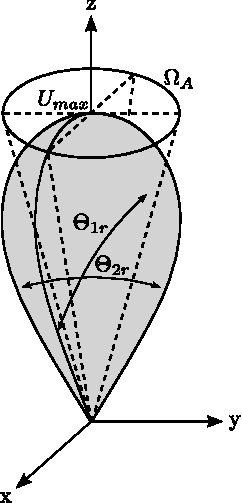
\includegraphics[scale = 1]{Figures/Intro/intro_4.pdf}
\caption{Ángulo sólido del haz.}
\label{fig_intro:4}
\end{figure}
%%%%
Con dicha aproximación, la expresión \eqref{ec_intro:21} se reduce a:
%%%%
\begin{align}
D_0 = \frac{4\pi}{\Omega_A} \simeq \frac{4\pi}{\Theta_{1r}\Theta_{2r}}
\label{ec_intro:23}
\end{align}
%%%%
El ángulo sólido del haz $\Omega_A$ se aproxima como:
%%%%
\begin{align}
\Omega_A \simeq \Theta_{1r}\Theta_{2r}
\tag{\ref{ec_intro:23}a}
\label{ec_intro:24}
\end{align}
%%%%
donde:
%%%%
\begin{align*}
\Theta_{1r} &= \text{Ancho de haz de potencia media en un plano (rad).}\\
\Theta_{2r} &= \text{Ancho de haz de potencia media en un plano en ángulo recto al otro (rad).}
\end{align*}
%%%%

%%%%
\subsection{Eficiencia}
\label{subsec_intro_eficien}
%%%%

%%%%
La \emph{eficiencia} es un parámetro utilizado para considerar las pérdidas producidas tanto en el terminal de entrada como en la estructura de la antena.

En términos generales, la eficiencia puede expresarse como:
%%%%
\begin{align}
e_0 = e_re_ce_d
\label{ec_intro:25}
\end{align}
%%%%
donde:
%%%%
\begin{align*}
e_0 = &\text{ Eficiencia total.}\\
e_g = &\,1 - \left|\Gamma\right|^2 = \text{Eficiencia por reflexiones, debida a la desadaptación de impedancias en}\\
&\text{ el terminal de entrada de la antena.}\\
e_c = &\text{ Eficiencia conductiva, debida a las pérdidas por efecto Joule.}\\
e_d = &\text{ Eficiencia dieléctrica, debida a las pérdidas dieléctricas.}
\end{align*}
%%%%
Usualmente, la eficiencia se determina considerando condiciones de adaptación ideales, por lo que $e_0$ suele expresarse como:
%%%%
\begin{align}
e_0 = e_r
\label{ec_intro:26}
\end{align}
%%%%
donde $e_r$ es la \emph{eficiencia de radiación de la antena}.
%%%%

%%%%
\subsection{Ganancia}
\label{subsec_intro_ganancia}
%%%%

%%%%
Se define como \emph{ganancia} a la relación entre la intensidad de radiación en una determinada dirección que produce un elemento radiante en el espacio y la intensidad de radiación que se obtendría si la potencia de entrada de la antena se irradiara isotrópicamente. La intensidad de radiación correspondiente a la potencia radiada isotrópicamente es igual a la potencia de entrada de la antena dividida por $4\pi$, por lo que la ganancia puede expresarse como:
%%%%
\begin{align}
G = 4\pi\frac{U}{P_{in}}
\label{ec_intro:27}
\end{align}
%%%%
Debido a las pérdidas existentes en la antena, la potencia radiada no será la misma que la potencia de entrada; es posible entonces relacionar ambas potencias mediante la eficiencia de radiación.
%%%%
\begin{align}
P_{rad} = e_rP_{in}
\label{ec_intro:28}
\end{align}
%%%%
La ganancia puede expresarse como:
%%%%
\begin{align}
G = e_r4\pi\frac{U}{P_{rad}}
\label{ec_intro:29}
\end{align}
%%%%
por lo que es posible relacionar la ganancia con la directividad.
%%%%
%%
\begin{align}
G = e_rD
\label{ec_intro:30}
\end{align}
%%
%%%%

%%%%
\subsection{Eficiencia del haz}
\label{subsec_intro_efi_haz}
%%%%

%%%%
La \emph{eficiencia del haz} $\varepsilon_M$ es un indicador del porcentaje de la potencia total radiada por la antena que se concentra en el haz principal. El ángulo sólido del haz está conformado por las contribuciones del lóbulo principal y de los lóbulos secundarios, por lo que:
%%%%
\begin{align}
\Omega_A = \Omega_M + \Omega_m
\label{ec_intro:31}
\end{align}
%%%%
donde:
%%%%
\begin{align*}
\Omega_M &= \text{Ángulo sólido del haz principal (sr).}\\
\Omega_m &= \text{Ángulo sólido de los haces laterales (sr).}
\end{align*}
%%%%
La eficiencia del haz, entonces, se define como:
%%%%
\begin{align}
\varepsilon_M = \frac{\Omega_M}{\Omega_A}
\label{ec_intro:32}
\end{align}
%%%%

%%%%
\subsection{Impedancia de entrada}
\label{subsec_intro_imp_ent}
%%%%

%%%%
La \emph{impedancia de entrada} se define como la impedancia que presenta la antena en sus terminales de entrada al circuito de alimentación. Generalmente es compleja, y puede expresarse como:
%%%%
\begin{align}
Z_A = R_A + jX_A
\label{ec_intro:33}
\end{align}
%%%%
donde:
%%%%
\begin{align*}
Z_A &= \text{Impedancia de entrada ($\Omega$).}\\
R_A &= \text{Resistencia de entrada ($\Omega$).}\\
X_A &= \text{Reactancia de entrada ($\Omega$).}
\end{align*}
%%%%
La parte resistiva de la impedancia de entrada está compuesta por dos componentes:
%%%%
\begin{align}
R_A = R_R +R_L
\label{ec_intro:34}
\end{align}
%%%%
donde:
%%%%
\begin{align*}
R_R &= \text{Resistencia de radiación de la antena ($\Omega$).}\\
R_L &= \text{Resistencia de pérdidas de la antena ($\Omega$).}
\end{align*}
%%%%
Si se asume que la antena es excitada con un generador con impedancia interna:
%%%%
\begin{align}
Z_G = R_G + jX_G
\label{ec_intro:35}
\end{align}
%%%%
donde:
%%%%
\begin{align*}
R_G &= \text{Resistencia de la impedancia del generador ($\Omega$).}\\
X_G &= \text{Reactancia de la impedancia del generador ($\Omega$).}
\end{align*}
%%%%
y la antena es usada como transmisora, puede representarse la antena y el generador por el circuito equivalente Thevenin de la figura \ref{fig_intro:5}.
%%%%
\begin{figure} [H]
\centering 
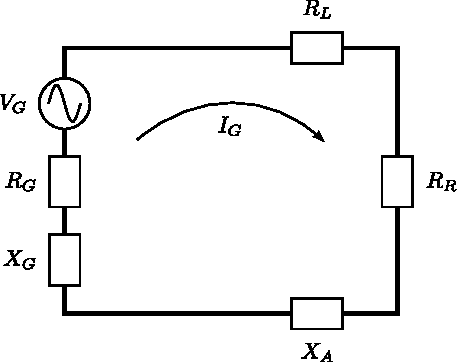
\includegraphics[scale = 1]{Figures/Intro/intro_5.pdf}
\caption{Circuito equivalente Thevenin de la antena en modo transmisora.}
\label{fig_intro:5}
\end{figure}
%%%%
Para determinar la potencia radiada (entregada a $R_R$) y la potencia disipada por efecto Joule (entragada a $R_L$), primero se determina la corriente que circula por el circuito equivalente, que  está dada por:
%%%%
\begin{align}
I_G = \frac{V_G}{Z_A + Z_G} = \frac{V_G}{\left(R_R + R_L + R_G\right) + j\left(X_A + X_G\right)}
\label{ec_intro:36}
\end{align}
%%%%
La potencia radiada por la antena está dada por:
%%%%
\begin{align}
P_R = \frac{1}{2}\left|I_G\right|^2R_R = \frac{\left|V_G\right|^2}{2}\left[\frac{R_R}{\left(R_R + R_L + R_G\right)^2 + \left(X_A + X_G\right)^2}\right]
\label{ec_intro:37}
\end{align}
%%%%
y la potencia disipada por efecto Joule por:
%%%%
\begin{align}
P_L = \frac{1}{2}\left|I_G\right|^2R_R = \frac{\left|V_G\right|^2}{2}\left[\frac{R_L}{\left(R_R + R_L + R_G\right)^2 + \left(X_A + X_G\right)^2}\right]
\label{ec_intro:38}
\end{align}
%%%%
La potencia restante se disipa sobre la resistencia interna del generador $R_G$, cuya expresión es:
%%%%
\begin{align}
P_G = \frac{1}{2}\left|I_G\right|^2R_R = \frac{\left|V_G\right|^2}{2}\left[\frac{R_G}{\left(R_R + R_L + R_G\right)^2 + \left(X_A + X_G\right)^2}\right]
\label{ec_intro:39}
\end{align}
%%%%
La máxima transferencia de potencia a la antena se produce cuando la impedancia de entrada de la antena es la conjugada de la impedancia interna del generador, o sea:
%%%%
\begin{gather}
R_R + R_L = R_G
\label{ec_intro:40}\\
X_A = - X_G
\label{ec_intro:41}
\end{gather}
%%%%
En este caso, las potencias involucradas son:
%%%%
\begin{align}
P_R &= \frac{\left|V_G\right|^2}{8}\left[\frac{R_R}{\left(R_R + R_L\right)^2}\right]
\label{ec_intro:42}\\
P_L &= \frac{\left|V_G\right|^2}{8}\left[\frac{R_L}{\left(R_R + R_L\right)^2}\right]
\label{ec_intro:43}\\
P_G &= \frac{\left|V_G\right|^2}{8}\left[\frac{1}{R_R + R_L}\right]
\label{ec_intro:44}
\end{align}
%%%%
Puede observarse que $P_G = P_R + P_L$, por lo que de la potencia provista por el generador, la mitad se disipa en la resistencia interna $R_G$ y la otra mitad es entregada a la antena, de la cual parte se disipa por efecto Joule y parte se irradia. Esta condición, la de máxima transferencia de potencia, se cumple cuando existe \emph{adaptación de impedancias}. Si la antena idealmente no tuviera pérdidas, el generador debería suministrar el doble de la potencia que se desea irradiar en la condición de máxima transferencia de potencia. En la práctica la potencia suministrada por el generador debe ser mayor, para compensar las pérdidas óhmicas tanto en la antena como en las líneas de transmisión. Una medida de las pérdidas en la antena surge a partir de la \emph{eficiencia de radiación}, que puede expresarse como:
%%%%
\begin{align}
e_r = \frac{R_R}{R_R + R_L}
\label{ec_intro:45}
\end{align}
%%%%

%%%%
\subsection{Area efectiva}
\label{subsec_intro_area_efec}
%%%%

%%%%
Cuando una antena se utiliza como receptora, recibe una determinada densidad de potencia de la onda incidente que convierte en potencia eléctrica. Se define como \emph{área efectiva} a la relación entre la potencia que la onda proporciona a una carga conectada a la antena receptora y la densidad de potencia de la onda incidente. El área efectiva puede expresarse como:
%%%%
\begin{align}
A_e = \frac{P_T}{W_i}
\label{ec_intro:46}
\end{align}
%%%%
donde:
%%%%
\begin{align*}
A_e &= \text{Área efectiva (m$^2$).}\\
P_T &= \text{Potencia proporcionada a la carga (W).}\\
W_i &= \text{Densidad de potencia de la onda incidente (W/m$^2$).}
\end{align*}
%%%%
Con el fin de entender claramente el concepto de área efectiva, en la figura \ref{fig_intro:6} se muestra el circuito equivalente Thevenin de una antena receptora conectada a una carga $Z_T$.
%%%%
\begin{figure} [H]
\centering 
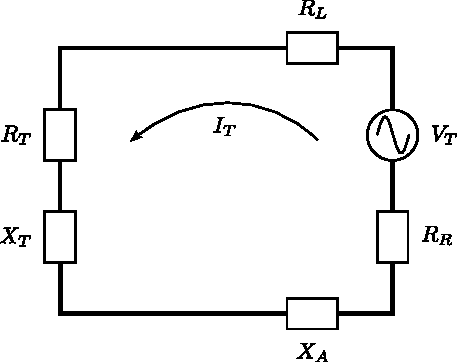
\includegraphics[scale = 1]{Figures/Intro/intro_6.pdf}
\caption{Circuito equivalente Thevenin de la antena en modo receptora.}
\label{fig_intro:6}
\end{figure}
%%%%
donde:
%%%%
\begin{align}
Z_T = R_T + jX_T
\label{ec_intro:47}
\end{align}
%%%%
La potencia proporcionada a la resistencia $R_T$ está dada por:
%%%%
\begin{align}
P_T = \frac{\left|V_T\right|^2}{2}\left[\frac{R_T}{\left(R_R + R_L + R_T\right)^2 + \left(X_A + X_T\right)^2}\right]
\label{ec_intro:48}
\end{align}
%%%%
y la potencia disipada por efecto Joule por:
%%%%
\begin{align}
P_L = \frac{\left|V_T\right|^2}{2}\left[\frac{R_L}{\left(R_R + R_L + R_T\right)^2 + \left(X_A + X_T\right)^2}\right]
\label{ec_intro:49}
\end{align}
%%%%
La potencia restante se dispersa al espacio, o sea, se disipa sobre la resistencia de radiación $R_R$, y su expresión es:
%%%%
\begin{align}
P_R = \frac{\left|V_T\right|^2}{2}\left[\frac{R_R}{\left(R_R + R_L + R_T\right)^2 + \left(X_A + X_T\right)^2}\right]
\label{ec_intro:50}
\end{align}
%%%%
En condiciones de adaptación, las potencias quedan expresadas como:
%%%%
\begin{align}
P_T &= \frac{\left|V_T\right|^2}{8R_T}
\label{ec_intro:51}\\
P_L &= \frac{\left|V_T\right|^2}{8}\left[\frac{R_L}{\left(R_R + R_L\right)^2}\right]
\label{ec_intro:52}\\
P_R &= \frac{\left|V_T\right|^2}{8}\left[\frac{R_R}{\left(R_R + R_L\right)^2}\right]
\label{ec_intro:53}
\end{align}
%%%%
y puede observarse que $P_T = P_R + P_L$. Para este caso, y si la antena está orientada para recibir máxima señal (es decir, orientada hacia donde la directividad es igual a la directividad máxima $D_0$), el área efectiva se denomina \emph{área efectiva máxima}. El área efectiva máxima está relacionada con el área física de la antena mediante la \emph{eficiencia de abertura}, cuya expresión es:
%%%%
\begin{align}
\varepsilon_{ap} = \frac{A_{em}}{A_p}
\label{ec_intro:54}
\end{align}
%%%%
donde:
%%%%
\begin{align*}
\varepsilon_{ap} &= \text{Eficiencia de abertura.}\\
A_{em} &= \text{Área efectiva máxima (m$^2$).}\\
A_p &= \text{Área física (m$^2$).}
\end{align*}
%%%%
Se cumplirá siempre que $0 \leq\varepsilon_{ap}\leq 1$. Si se asumen pérdidas por efecto Joule nulas ($R_L = 0$), la potencia entregada a la carga será igual a la potencia que la antena dispersa en el espacio, o sea, habrá una potencia reirradiada exactamente igual a la recibida.

Para determinar la relación entre el área efectiva máxima y la directividad, se parte de un enlace entre dos antenas, físicamene ubicadas en el espacio libre y separadas por una distancia $R$, como se muestra en la figura \ref{fig_intro:7}.
%%%%
\begin{figure} [H]
\centering 
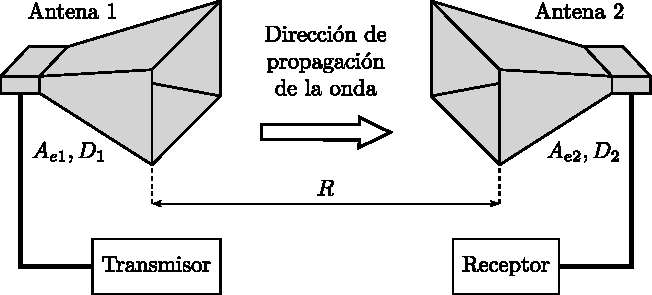
\includegraphics[scale = 1]{Figures/Intro/intro_7.pdf}
\caption{2 antenas separadas por una distancia $R$.}
\label{fig_intro:7}
\end{figure}
%%%%
En primera instancia, se asume que la antena 1 es la transmisora y la antena 2 es la receptora. La densidad de potencia radiada por la antena 1 a una distancia $R$ responde a la expresión:
%%%%
\begin{align}
W_1 = \frac{P_TD_1}{4\pi R^2}
\label{ec_intro:55}
\end{align}
%%%%
La potencia recibida por la antena 2 es:
%%%%
\begin{align}
P_2 = A_{e2}W_1 = A_{e2}\frac{P_TD_1}{4\pi R^2}
\label{ec_intro:56}
\end{align}
%%%%
por lo que:
%%%%
\begin{align}
D_1A_{e2} = \frac{P_2}{P_T}\,4\pi R^2
\tag{\ref{ec_intro:56}a}
\label{ec_intro:57}
\end{align}
%%%%
Si ahora la antena 2 es usada como transmisora y la antena 1 como receptora, puede expresarse que:
%%%%
\begin{align}
D_2A_{e1} = \frac{P_1}{P_T}\,4\pi R^2
\label{ec_intro:58}
\end{align}
%%%%
por lo que a partir de las expresiones \eqref{ec_intro:57} y \eqref{ec_intro:58} se llega a:
%%%%
\begin{align}
\frac{D_1}{A_{e1}} = \frac{D_2}{A_{e2}}
\label{ec_intro:59}
\end{align}
%%%%
El incremento de la directividad genera un aumento del área efectiva, por lo que:
%%%%
\begin{align}
\frac{D_{01}}{A_{em1}} = \frac{D_{02}}{A_{em2}}
\label{ec_intro:60}
\end{align}
%%%%
Suponiendo que la antena 1 es un foco isotrópico, su directividad sería unitaria, por lo que:
%%%%
\begin{align}
A_{em1} = \frac{A_{em2}}{D_{02}}
\label{ec_intro:61}
\end{align}
%%%%
Considerando ahora que la antena 2 es un dipolo de Hertz, su área efectiva máxima, asumiendo que las pérdidas óhmicas son nulas, está expresada por:
%%%%
\begin{align}
A_{em} = \frac{\left|V_T\right|^2}{8W_iR_R}
\label{ec_intro:62}
\end{align}
%%%%
Como el dipolo es muy corto, puede asumirse que el campo inducido es constante y de fase uniforme, por lo que la tensión inducida es:
%%%%
\begin{align}
V_T = El
\label{ec_intro:63}
\end{align}
%%%%
donde:
%%%%
\begin{align*}
V_T &= \text{Tensión inducida en el dipolo (V).}\\
E &= \text{Campo eléctrico de la onda incidente (V/m).}\\
l &= \text{Longitud del dipolo (m).}
\end{align*}
%%%%
Para una onda incidente plana, la densidad de potencia incidente puede expresarse como:
%%%%
\begin{align}
W_i = \frac{E^2}{2\eta}
\label{ec_intro:64}
\end{align}
%%%%
La resistencia de radiación del dipolo de Hertz está dada por \cite{Fano2}:
%%%%
\begin{align}
R_R = 80\left(\frac{\pi l}{\lambda}\right)^2
\label{ec_intro:65}
\end{align}
%%%%
El área efectiva máxima, entonces, puede expresarse como:
%%%%
\begin{align}
A_{em} = \frac{\left(El\right)^2}{8\,\dfrac{E^2}{2\eta}\,80\left(\dfrac{\pi l}{\lambda}\right)^2} = \frac{3\lambda^2}{8\pi}
\label{ec_intro:66}
\end{align}
%%%%
Para un dipolo de Hertz, la directividad máxima es \cite{Fano2}:
%%%%
\begin{align}
D_0 = \frac{3}{2}
\label{ec_intro:67}
\end{align}
%%%%
Puede entonces determinarse el área efectiva máxima de un foco isotrópico, cuya expresión final es:
%%%%
\begin{align}
A_{em} = \frac{\lambda^2}{4\pi}
\label{ec_intro:68}
\end{align}
%%%%
En forma general, entonces, puede expresarse el área efectiva máxima en función de la directividad máxima $D_0$ mediante la expresión:
%%%%
\begin{align}
A_{em} = \frac{\lambda^2}{4\pi}D_0
\label{ec_intro:69}
\end{align}
%%%%
Si existen pérdidas óhmicas y dieléctricas en la antena, su área efectiva máxima debe modificarse para tener en cuenta tales pérdidas, por lo que:
%%%%
\begin{align}
A_{em} = e_r\frac{\lambda^2}{4\pi}D_0 = \frac{\lambda^2}{4\pi}G_0
\label{ec_intro:70}
\end{align}
%%%%

%%%%
\subsection{Polarización}
\label{subsec_intro_polar}
%%%%

Se define como \emph{polarización de una onda electromagnética} a la dirección del vector intensidad del campo eléctrico $\mathbf{E}$, o sea, la dirección en la cual el campo eléctrico varía temporalmente.

El campo eléctrico $\mathbf{E}$ puede expresarse como la suma de dos componentes ortogonales $E_x$ y $E_y$, con una diferencia de fase temporal $\delta$ entre las mismas, es decir:
%%%%
\begin{align}
\mathbf{E} = E_x\,\versor{x} + E_y\,\versor{y} =  E_{0x}\cos\left(\omega t\right)\versor{x} + E_{0y}\cos\left(\omega t + \delta\right)\versor{y}
\label{ec_intro:71}
\end{align}
%%%%
donde:
%%%%
\begin{align*}
E_{0x} &= \text{Amplitud de la componente }E_x\text{ (V/m).}\\
E_{0y} &= \text{Amplitud de la componente }E_y\text{ (V/m).}
\end{align*}
%%%%
Ambas componentes son perpendiculares a la dirección de propagación, que coincide con la dirección del eje \emph{z}.

Las polarizaciones más comúnmente empleadas en la práctica son:
%%%%
\begin{enumerate}
\item Polarización lineal vertical: El campo eléctrico varía temporalmente sobre el eje \emph{y} al propagarse, por lo que la expresión resultante del campo eléctrico $\mathbf{E}$ es:
%%%%
\begin{align}
\mathbf{E} = E_y\,\versor{y} =  E_{0y}\cos\left(\omega t\right)\versor{y}
\label{ec_intro:72}
\end{align}
%%%%
\item Polarización lineal horizontal: El campo eléctrico varía temporalmente sobre el eje \emph{x} al propagarse, por lo que la expresión resultante del campo eléctrico $\mathbf{E}$ es:
%%%%
\begin{align}
\mathbf{E} = E_x\,\versor{x} =  E_{0x}\cos\left(\omega t\right)\versor{x}
\label{ec_intro:73}
\end{align}
%%%%
\item Polarización circular: El campo eléctrico varía temporalmente describiendo una circunsferencia al propagarse, por lo que la expresión resultante del campo eléctrico $\mathbf{E}$ es:
%%%%
\begin{align}
\mathbf{E} = E_x\,\versor{x} + E_y\,\versor{y} =  E_{0}\cos\left(\omega t\right)\versor{x} \pm E_{0}\sen\left(\omega t\right)\versor{y}
\label{ec_intro:74}
\end{align}
%%%%
Para que la polarización sea circular, debe cumplirse que:
%%%%
\begin{align}
E_{0x} &= E_{0y} = E_0
\label{ec_intro:75}\\
\delta &= \pm\left(2n + 1\right)\dfrac{\pi}{2}
\label{ec_intro:76}
\end{align}
%%%%
\end{enumerate}
%%%%
En la práctica, las antenas se diseñan para que trabajen con una determinada polarización; cualquier componente existente con otra polarización no es deseada y debe ser lo menor posible. A tal efecto, se define:
%%%%
\begin{itemize}
\item Copolarización: Es la componente del campo eléctrico $\mathbf{E}$ con la polarización deseada.
\item Polarización cruzada: Es la componente del campo eléctrico $\mathbf{E}$ cuya polarización no es la deseada y que es ortogonal a la copolarización.
\end{itemize}
%%%%
Si la antena es diseñada para que trabaje con polarización lineal vertical, es decir, que la copolarización se corresponda con la polarización en el eje \emph{y}, la polarización cruzada corresponderá a las componentes del campo eléctrico $\mathbf{E}$ con polarización en el eje \emph{x}.

Para determinar la relación entre las amplitudes de las componentes ortogonales de polarización lineal, se define la \emph{relación de polarización lineal} $\rho_L$ \cite{Fano2}, o simplemente \emph{relación de polarización cruzada}, cuya expresión es:
%%%%
\begin{align}
\rho_L &= \dfrac{E_{0y}}{E_{0x}}
\label{ec_intro:77}
\end{align}
%%%%
En dB, la expresión \eqref{ec_intro:77} resulta:
%%%%
\begin{align}
\rho_L &= 20\log\left(E_{0y}\right) -  20\log\left(E_{0x}\right)
\label{ec_intro:78}
\end{align}
%%%%